% !TEX program = pdflatex
%% IEEE Journal of Biomedical and Health Informatics (J-BHI) Manuscript
%% Template: IEEEtran (journal mode)
%%
%% Title: Physics-Informed Deep Learning for Generalizable Gait Kinetics in
%%        Assistive Exoskeletal Robotics via Speed-Conditioned State-Space Models
%%
%% Target: IEEE J-BHI Special Issue -- "Emerging AI Paradigms for Next-Gen
%%         Medicine: Safety, Reliability, and Digital Twins"
%% Deadline: 30 September 2026

\documentclass[journal]{IEEEtran}

% Custom command for the impulse response kernel
\newcommand{\Kbar}{\bar{\mathbf{K}}}
\newcommand{\Abar}{\bar{\mathbf{A}}}
\newcommand{\Bbar}{\bar{\mathbf{B}}}

% ========================== PACKAGES ===========================
\usepackage[T1]{fontenc}
\usepackage[utf8]{inputenc}
\usepackage{amsmath,amssymb,amsfonts}
\usepackage{algorithmic}
\usepackage{graphicx}
\usepackage{textcomp}
\usepackage{xcolor}
\usepackage{booktabs}
\usepackage{multirow}
\usepackage{siunitx}
\usepackage{hyperref}
\usepackage{cite}
\usepackage{array}
\usepackage{subcaption}
\usepackage{balance}

% Graphics path
\graphicspath{{figures/}}

% SI units setup
\sisetup{
  per-mode=symbol,
  inter-unit-product=\ensuremath{{}\cdot{}},
  separate-uncertainty=true,
}

% Custom commands
\newcommand{\lm}{l_{\mathrm{m}}}
\newcommand{\vm}{v_{\mathrm{m}}}
\newcommand{\dmodel}{d_{\mathrm{model}}}
\newcommand{\dstate}{d_{\mathrm{state}}}
\newcommand{\Fz}{F_z}
\newcommand{\dotq}{\dot{q}}
\newcommand{\tauhat}{\hat{\tau}}
\newcommand{\lamjerk}{\lambda_{\mathrm{jerk}}}
\newcommand{\lampower}{\lambda_{\mathrm{power}}}
\newcommand{\Nmskg}{\si{\newton\metre\per\kilogram}}
\newcommand{\Nmskgsq}{\si{\newton\metre\per\kilogram\per\second\squared}}
\newcommand{\Wkg}{\si{\watt\per\kilogram}}

% Float spacing tuning for compact IEEE layout
\setlength{\textfloatsep}{2.5pt plus 1pt minus 1pt}
\setlength{\floatsep}{2.5pt plus 1pt minus 1pt}
\setlength{\intextsep}{2.5pt plus 1pt minus 1pt}
\setlength{\dbltextfloatsep}{3pt plus 1pt minus 1pt}
\setlength{\dblfloatsep}{2.5pt plus 1pt minus 1pt}
\setlength{\abovecaptionskip}{1.5pt plus 1pt minus 1pt}
\setlength{\belowcaptionskip}{1.5pt plus 1pt minus 1pt}
\renewcommand{\topfraction}{0.95}
\renewcommand{\bottomfraction}{0.95}
\renewcommand{\textfraction}{0.05}
\renewcommand{\dbltopfraction}{0.95}
\renewcommand{\dblfloatpagefraction}{0.90}
\setcounter{topnumber}{3}
\setcounter{dbltopnumber}{3}


% ========================== DOCUMENT ===========================
\begin{document}

% ========================== TITLE ==============================
\title{Physics-Informed Deep Learning for Generalizable Gait Kinetics in Assistive Exoskeletal Robotics via Speed-Conditioned State-Space Models}

\author{Muhammad~Mujeeb~Ur~Rahman%
\thanks{Manuscript submitted September 2026. This work was performed independently and did not receive external commercial funding.}%
\thanks{M.~M.~U.~Rahman is an independent researcher specializing in biomedical artificial intelligence and biomechatronic systems (e-mail: mujeebbadwan1155@gmail.com).}}

\markboth{IEEE Journal of Biomedical and Health Informatics}%
{Rahman: Physics-Informed SSM for Exoskeletal Gait Kinetics}

\maketitle
\IEEEpeerreviewmaketitle

% ========================== ABSTRACT ===========================
\begin{abstract}
Data-driven gait joint-kinetics prediction often fails to generalize across walking velocities and produces non-smooth torque trajectories that risk user discomfort and control instability in robotic exoskeletons and active prostheses. We propose a physics-guided diagonal state-space model (S4D) combining Feature-wise Linear Modulation (FiLM) speed conditioning with auxiliary torque-jerk and mechanical power consistency regularization. Evaluated on a primary multi-speed dataset (44 subjects, 0.6--1.6~\si{\metre\per\second}) and benchmarked against parameter-matched bidirectional LSTM and dilated Temporal Convolutional Network (TCN) baselines, our architecture achieves an overall mean absolute error (MAE) of $0.0765 \pm 0.0032$~\Nmskg{} ($0.0742 \pm 0.0008$~\Nmskg{} for Model~2 without physics penalty) and Pearson correlation $r = 0.9438 \pm 0.0040$ ($r = 0.9466 \pm 0.0020$ for Model~2). In leave-one-speed-out cross-validation, bidirectional baselines dominate cross-speed accuracy (BiLSTM MAE: 0.0575~\Nmskg{}), while within causal S4D variants Model~2 attains lowest MAE (0.0664~\Nmskg{}). Crucially, auxiliary physics regularization in Model~3 suppresses high-frequency torque oscillations, achieving a 25--34\% jerk reduction across speed folds (averaging 29.5\%, subject-level paired $p = 0.0027$, trial-level $p < 10^{-12}$, Cohen's $d_z = -1.650$) at an accuracy trade-off of 7.1\% cross-speed MAE (0.0711 vs.\ 0.0664~\Nmskg{}). Under zero-shot transfer to the independent Fukuchi~et~al. dataset (42 subjects, 328 trials), Dilated TCN attains highest overall transfer ($r = 0.8347$, MAE 0.2268~\Nmskg{}), while within S4D FiLM conditioning improves correlation from $r = 0.6553$ to $0.7492$ (a 14.3\% gain). Exported to ONNX, the 189,699-parameter model executes in 9.93~\si{\milli\second} on a host CPU. This work establishes an accurate, smooth, and edge-deployable foundation for assistive biomechatronic controllers.
\end{abstract}

\begin{IEEEkeywords}
Gait analysis, state-space models, physics-informed deep learning, joint kinetics, speed generalization, wearable robotics, transfer learning, biomechanical surrogate.
\end{IEEEkeywords}

% ========================== I. INTRODUCTION ====================
\section{Introduction}
\IEEEPARstart{A}{ccurate} prediction of lower-limb joint kinetics---the net moments at the hip, knee, and ankle---is fundamental for real-time control of powered exoskeletons, active prostheses, and intelligent orthoses~\cite{lim2019review}. Discrepancies lead to inappropriate actuator forces that increase metabolic expenditure, compromise stability, and pose safety hazards~\cite{tucker2015control}.

Contemporary ML models (LSTMs, TCNs, Transformers) achieve impressive accuracy under matched conditions~\cite{mundt2020prediction, johnson2021comparison, sharifi2023biomat} but face three limitations: (1) poor speed generalization---everyday walking spans 0.6--1.6~\si{\metre\per\second}~\cite{bohannon2011comfortable}; (2) physically implausible, jerky outputs lacking inductive biases~\cite{dorschky2019cnn, stanev2020learning}---high torque chattering is hypothesized to excite spastic reflexes and induce painful skin shear in neuro-rehabilitation~\cite{baud2021review}; (3) computational complexity for wearable controllers~\cite{goel2022s, young2017state}.

Structured state-space models (SSMs), particularly diagonal S4D~\cite{gu2022parameterization}, provide a compelling paradigm. HiPPO-initialized diagonal S4D achieves long-range temporal modeling with linear complexity and fixed recurrent state memory~\cite{goel2022s}.

We propose a physics-guided S4D unifying speed-conditioned temporal modeling with biomechanical safety constraints (Fig.~\ref{fig:architecture}): (1) four-layer S4D backbone ($\dmodel=64$, $\dstate=64$) in pure PyTorch for ONNX export; (2) post-block FiLM speed conditioning~\cite{perez2018film} for velocity-dependent modulation; (3) torque-jerk minimization and instantaneous joint mechanical power consistency losses.

Validated on a six-speed treadmill dataset (44 subjects, 262 trials) and zero-shot on Fukuchi~et~al.~\cite{fukuchi2018public} (42 subjects, 328 trials) via anti-leakage LOSO, FiLM conditioning and physics guidance serve complementary purposes.

Our \textbf{Dual-Use Operational Paradigm} aligns with \emph{Safety, Reliability, and Digital Twins}~\cite{chakshu2024digital, sun2023digital}: (1) \textbf{Clinical Biomechanical Surrogate Mode:} In laboratory or clinical gait analysis, the model acts as an ultrafast surrogate for dynamic optimization and inverse dynamics (reducing minutes of simulation to 9.93~ms per stride cycle), leveraging scaled musculoskeletal states for subject-specific kinetic estimation. (2) \textbf{Wearable Robotics Roadmap:} For closed-loop assistive devices, the diagonal continuous-time SSM formulation provides a theoretical foundation for $\mathcal{O}(1)$ streaming torque targets, with current offline deployment benchmarked on stride-normalized inputs.

Principal contributions: (1) We establish a functional decoupling between velocity conditioning and physical regularization: FiLM drives domain generalization and cross-speed adaptation within S4D, while physics losses provide substantial jerk reduction (25--34\%, averaging 29.5\%, subject-level paired $p = 0.0027$, trial-level $p < 10^{-12}$). (2) We complete a systematic $2 \times 2$ factorial ablation (Model~1.5 without FiLM) confirming that torque smoothing operates independently of speed conditioning. (3) We benchmark against parameter-matched baseline Model~1 (172k params) alongside BiLSTM (173k params) and Dilated TCN (171k params) architectures (with Models~2 and 3 adding 17k parameters for FiLM modulation), transparently detailing trade-offs where bidirectional baselines achieve superior cross-speed MAE while S4D provides causal efficiency. (4) We enforce a strict, firewalled leave-one-speed-out (LOSO) protocol guaranteeing zero velocity leakage, paired with zero-shot cross-dataset evaluation across 328 independent trials.

% ========================== II. RELATED WORK ===================
\section{Related Work}

\subsection{Data-Driven Gait Kinetics Prediction}
Early work used shallow ANNs and wavelets~\cite{ardestani2014human}. LSTMs and BiLSTMs became standard for temporal gait dynamics~\cite{mundt2020prediction, johnson2021comparison}. TCNs and Transformers capture multi-joint synergies and long-range dependencies~\cite{molinaro2024estimating, sharifi2023biomat, hossain2023estimation} but degrade outside training speeds~\cite{camargo2021machine}.

\subsection{Physics-Informed Deep Learning in Biomechanics}
PINNs prevent kinematically impossible predictions~\cite{karniadakis2021physics}. Approaches range from differentiable simulators~\cite{werling2021fast} to soft penalty losses~\cite{dorschky2019cnn, stanev2020learning}. Differentiable simulation faces numerical stiffness and convergence issues~\cite{werling2021fast}; soft auxiliary losses offer a robust compromise~\cite{dorschky2019cnn}.

\subsection{State-Space Models for Sequential Modeling}
SSMs are efficient alternatives to Transformers and RNNs across continuous sequential domains~\cite{goel2022s, gu2022parameterization}. Rooted in control theory, SSMs map $x(t)$ to hidden states $\mathbf{h}(t)$ via linear differential equations with HiPPO-initialized transition matrices. Diagonal S4D~\cite{gu2022parameterization} simplifies computation while retaining capacity. S5~\cite{smith2023s5} and Mamba~\cite{gu2024mamba} add multi-input formulations and selective gating. We use S4D for its time-invariant diagonal representation enabling exact 1D convolutional training and ONNX export without custom kernels.

\subsection{Speed Conditioning in Locomotion Modeling}
Walking velocity systematically alters gait dynamics~\cite{bohannon2011comfortable}. FiLM~\cite{perez2018film} introduces affine transformations conditioned on context variables, enabling unified networks to adapt across continuous speeds.

\subsection{Domain Generalization and Distribution Shift in Biomechanics}
Distribution shift across cohorts, sensors, and protocols is a persistent challenge~\cite{halilaj2018machine, gholami2020subject}. Within-lab evaluations report misleadingly optimistic performance~\cite{mundt2021estimation}. Robust generalization requires expressive representations maintaining physical realism under covariate shift~\cite{young2017state}. Zero-shot cross-dataset transfer serves as the ultimate test for biomechanical surrogates.

% --- Figure 1: Architecture ---
\begin{figure*}[!t]
\centering
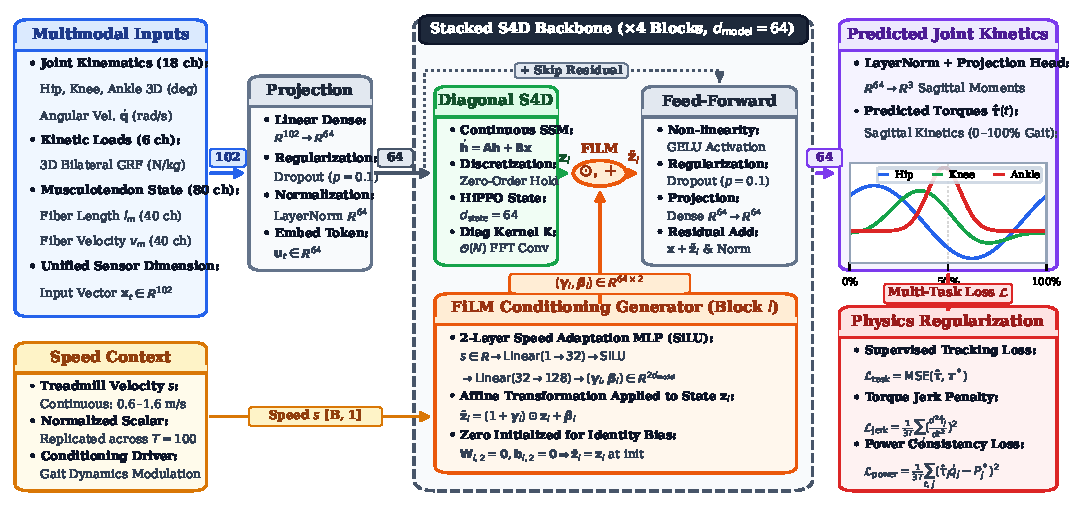
\includegraphics[width=0.82\textwidth]{fig1_architecture.pdf}
\caption{Architectural pipeline of the proposed physics-guided diagonal state-space model (S4D) with FiLM speed conditioning and auxiliary loss regularization. Multimodal inputs (102 channels across normalized gait cycle $T=100$) are projected to $\dmodel=64$ and processed through 4 stacked S4D blocks. Each block features an independent 2-layer FiLM MLP that dynamically modulates hidden activations according to walking speed $s$. Auxiliary torque-jerk and power consistency loss terms regularize outputs during training.}
\label{fig:architecture}
\end{figure*}

% ========================== III. METHODS =======================
\section{Methods}

\subsection{Problem Formulation}
Given a temporal sequence of multimodal gait measurements $\mathbf{X} \in \mathbb{R}^{T \times D_{\mathrm{in}}}$ ($T=100$) comprising lower-limb joint kinematics, ground reaction forces, OpenSim-derived musculotendon states, and a walking-speed scalar $s \in \mathbb{R}$, our objective is to predict sagittal-plane joint moments $\hat{\boldsymbol{\tau}} \in \mathbb{R}^{T \times 3}$ for hip flexion/extension, knee flexion/extension, and ankle plantar/dorsiflexion. Ground-truth moments $\boldsymbol{\tau}^* \in \mathbb{R}^{T \times 3}$ are obtained from inverse dynamics and normalized by body mass (\Nmskg{}).

\subsection{Input Feature Representation}
\label{sec:features}
The input feature vector at each time step consists of $D_{\mathrm{in}} = 102$ continuous channels: (1)~\textbf{joint angles} (9 channels: 3D hip, knee, ankle in degrees); (2)~\textbf{angular velocities} (9 channels: numerical time-derivatives in \si{\radian\per\second}); (3)~\textbf{ground reaction forces} (3 channels: mass-normalized 3D GRF, zero during swing); (4)~\textbf{musculotendon lengths} $\lm$ (40 channels: extracted via OpenSim Muscle Analysis~\cite{delp2007opensim} on a scaled Rajagopal model~\cite{rajagopal2016opensim}); (5)~\textbf{musculotendon velocities} $\vm$ (40 channels: first time-derivatives in \si{\metre\per\second}); and (6)~\textbf{walking speed} (1 channel: treadmill velocity in \si{\metre\per\second} replicated across time). All features are z-score normalized using statistics computed strictly on the training partition.

\emph{Biomechanical Rationale for Musculotendon Features:} The inclusion of OpenSim-derived musculotendon lengths ($\lm$) and velocities ($\vm$) provides biophysical geometric priors reflecting Hill-type muscle-tendon operating paths. While active muscular force requires activation or EMG signals not present in kinematic datasets, incorporating geometric fiber excursions and contraction velocities derived from subject-scaled anatomical models decouples surface joint angles from internal anatomical configurations~\cite{delp2007opensim}.

\emph{Dynamic Bilateral GRF Body Mass Estimation:} Subject body mass $M$ is derived dynamically from steady-state vertical ground reaction force summed across both limbs ($F_z(t) = F_{z,\mathrm{left}}(t) + F_{z,\mathrm{right}}(t)$) averaged across complete strides:
\begin{equation}
    M = \frac{1}{g \cdot T_{\mathrm{stride}}} \int_0^{T_{\mathrm{stride}}} F_z(t) \, dt
    \label{eq:mass}
\end{equation}
where $g = 9.81$~\si{\metre\per\second\squared}. Over periodic steady-state gait, total vertical impulse equals total body weight ($M g$). This bilateral derivation was verified against 21 subjects with usable quiet-standing force-plate records, showing near-perfect agreement ($r = 0.9991$, $R^2 = 0.9981$, mean absolute difference 1.39~\si{\kilogram}, RMSE 1.48~\si{\kilogram}).

\emph{Musculoskeletal Model Scaling:} Musculoskeletal scaling is performed via OpenSim's \texttt{ScaleSet} API using anatomical segment length ratios derived from static calibration marker distances (pelvis width, femur, tibia, foot lengths, and torso height) on the Rajagopal model~\cite{rajagopal2016opensim}. Leg length (74.4--108.4~\si{\centi\metre}) correlated strongly with mean musculotendon length ($r = 0.9723, p < 10^{-27}$), confirming physiological scaling consistency.

\subsection{Model Architecture}
\label{sec:model}

\subsubsection{Diagonal State-Space Layer (S4D)}
Each S4D layer models continuous temporal evolution via a linear dynamical system:
\begin{align}
    \dot{\mathbf{h}}(t) &= \mathbf{A} \mathbf{h}(t) + \mathbf{B} x(t) \label{eq:ssm_h} \\
    y(t) &= \mathbf{C} \mathbf{h}(t) + \mathbf{D} x(t) \label{eq:ssm_y}
\end{align}
where $\mathbf{A} \in \mathbb{C}^{N \times N}$ is constrained to be diagonal ($N = \dstate = 64$), and $\mathbf{B} \in \mathbb{C}^{N \times 1}$, $\mathbf{C} \in \mathbb{C}^{1 \times N}$, $\mathbf{D} \in \mathbb{R}$. Continuous parameters are discretized via the zero-order hold (ZOH) method with timescale step size $\Delta$:
\begin{align}
    \Abar &= \exp(\Delta \mathbf{A}) \label{eq:zoh_a} \\
    \Bbar &= (\exp(\Delta \mathbf{A}) - \mathbf{I}) \mathbf{A}^{-1} \mathbf{B} \label{eq:zoh_b}
\end{align}
Because $\mathbf{A}$ is diagonal, $\Abar$ and $\Bbar$ are computed analytically via scalar element-wise operations without matrix inversion. The diagonal structure decouples the state recurrence into $N$ scalar equations, evaluated during training as a 1D convolution with the \textbf{impulse response convolution kernel}:
\begin{equation}
    \Kbar = \left(\mathbf{C}\Bbar,\, \mathbf{C}\Abar\Bbar,\, \mathbf{C}\Abar^2\Bbar,\, \dots,\, \mathbf{C}\Abar^{T-1}\Bbar\right) \in \mathbb{R}^T
    \label{eq:kernel}
\end{equation}
Because $\Abar$ is diagonal, the kernel $\Kbar$ is evaluated analytically in $\mathcal{O}(T \cdot \dstate)$ time via direct element-wise exponentiation, followed by standard 1D convolution, avoiding custom CUDA kernels and enabling parallel training. On stride-normalized cycles ($T=100$), evaluation uses causal 1D depthwise convolution; in continuous-time streaming, diagonal SSMs mathematically admit $\mathcal{O}(1)$ step-wise recurrent updates.

\subsubsection{FiLM Speed Conditioning Module}
To condition temporal dynamics on gait speed $s \in \mathbb{R}$, each S4D block $l \in \{1, \dots, 4\}$ incorporates an independent two-layer multi-layer perceptron:
\begin{equation}
    (\boldsymbol{\gamma}_l, \boldsymbol{\beta}_l) = \mathbf{W}_{l,2} \, \mathrm{SiLU}(\mathbf{W}_{l,1} s + \mathbf{b}_{l,1}) + \mathbf{b}_{l,2}
    \label{eq:film_mlp}
\end{equation}
where $\mathbf{W}_{l,1} \in \mathbb{R}^{32 \times 1}$, $\mathbf{W}_{l,2} \in \mathbb{R}^{2\dmodel \times 32}$, producing scale and shift vectors $\boldsymbol{\gamma}_l, \boldsymbol{\beta}_l \in \mathbb{R}^{\dmodel}$. The final weights $\mathbf{W}_{l,2}$ and biases $\mathbf{b}_{l,2}$ are initialized to zero, ensuring that the module begins as an identity operator:
\begin{equation}
    \tilde{\mathbf{z}}_l = (1 + \boldsymbol{\gamma}_l) \odot \mathbf{z}_l + \boldsymbol{\beta}_l
    \label{eq:film_modulation}
\end{equation}
where $\mathbf{z}_l \in \mathbb{R}^{T \times \dmodel}$ is the output activation of the $l$-th S4D block, and $\odot$ represents channel-wise broadcasting.

\subsubsection{Complete Backbone}
The architecture comprises: (1)~a linear input projection $\mathbb{R}^{102} \to \mathbb{R}^{64}$ with dropout ($p = 0.1$); (2)~four stacked S4D blocks ($d_{\mathrm{model}}=64, d_{\mathrm{state}}=64$, expansion ratio 2), each containing layer normalization, S4D layer, GELU non-linearity, linear feedforward network with skip residual connection, followed by post-block FiLM speed modulation in Models~2 and 3; and (3)~layer normalization followed by a linear prediction head $\mathbb{R}^{64} \to \mathbb{R}^3$ outputting predicted moments $\hat{\boldsymbol{\tau}}(t)$.
Model~1 (S4D Baseline) comprises 172,547 trainable parameters, matching the baseline parameter budgets. Models~2 and 3 add 17,152 parameters across four FiLM MLPs (totaling 189,699 trainable parameters) and export to a 0.53~MB ONNX file.

\subsection{Loss Functions}
\label{sec:loss}

\subsubsection{Supervised Task Loss}
The primary objective is the mean squared error (MSE) across time and joints:
\begin{equation}
    \mathcal{L}_{\mathrm{task}} = \frac{1}{3T} \sum_{t=1}^{T} \sum_{j=1}^{3} \left( \hat{\tau}_j(t) - \tau_j^*(t) \right)^2
    \label{eq:loss_task}
\end{equation}

\subsubsection{Torque Acceleration and Jerk Minimization Penalty}
To penalize rapid torque fluctuations and high-frequency force spikes, we incorporate a discrete second-derivative penalty (Equation~\ref{eq:loss_jerk}). While termed ``torque jerk'' following wearable robotics convention~\cite{baud2021review}, this metric physically represents the second time-derivative of joint moment ($\ddot{\tau}$, more precisely termed \emph{torque acceleration}):
\begin{equation}
    \mathcal{L}_{\mathrm{jerk}} = \frac{1}{3T} \sum_{t=1}^{T} \sum_{j=1}^{3} \left( \frac{d^2 \hat{\tau}_j(t)}{dt^2} \right)^2
    \label{eq:loss_jerk}
\end{equation}
where the second time-derivative is computed via discrete central finite differences:
\begin{equation}
    \frac{d^2 \hat{\tau}_j(t)}{dt^2} \approx \frac{\hat{\tau}_j(t+\Delta t) - 2\hat{\tau}_j(t) + \hat{\tau}_j(t-\Delta t)}{(\Delta t)^2}
    \label{eq:finite_diff}
\end{equation}
for $1 < t < T$, with one-sided second differences applied at boundaries ($t=1$ and $t=T$). The physical time step $\Delta t = T_{\mathrm{stride}} / (T - 1)$ is derived from stride durations extracted via anterior-posterior heel marker trajectory peak detection~\cite{zeni2008two}. The physical jerk root-mean-square (RMS) reported in evaluation tables corresponds directly to $\sqrt{\mathcal{L}_{\mathrm{jerk}}}$.

\subsubsection{Instantaneous Joint Mechanical Power Consistency Loss}
The power consistency loss penalizes discrepancies between the instantaneous mechanical joint power implied by predicted moments and the ground-truth inverse-dynamics joint power:
\begin{equation}
    \mathcal{L}_{\mathrm{power}} = \frac{1}{3T} \sum_{t=1}^{T} \sum_{j=1}^{3} \left( s_j \cdot \hat{\tau}_j(t) \cdot \dotq_j(t) - P_j^{\mathrm{meas}}(t) \right)^2
    \label{eq:loss_power}
\end{equation}
where $\mathbf{s} = [1, -1, -1]$ accounts for OpenSim coordinate sign definitions (hip flexion is mutually positive, whereas knee extension and ankle plantarflexion coordinate systems require sign reflection relative to angular velocity derivatives to match physiological work). Because $P_j^{\mathrm{meas}}(t) = s_j \tau_j^*(t) \dotq_j(t)$, the residual simplifies to $(\hat{\tau}_j(t) - \tau_j^*(t))^2 \dotq_j(t)^2$, representing an angular-velocity-squared weighted surrogate regularizer rather than an active energy-conserving invariant. This prioritizes rapid motion phases (e.g., ankle push-off at $\sim$3.5~\Wkg{} and knee damping) where torque fidelity most heavily dictates actuator power transfer and metabolic cost~\cite{winter2009biomechanics}.

\subsubsection{Total Combined Objective}
The overall multi-task objective is:
\begin{equation}
    \mathcal{L} = \mathcal{L}_{\mathrm{task}} + \lamjerk \, \mathcal{L}_{\mathrm{jerk}} + \lampower \, \mathcal{L}_{\mathrm{power}}
    \label{eq:loss_total}
\end{equation}
with $\lamjerk = 10^{-8}$ and $\lampower = 0.01$ selected from three candidate configurations ($\lambda_{\mathrm{jerk}} \in \{10^{-6}, 10^{-7}, 10^{-8}\}$, $\lambda_{\mathrm{power}} \in \{0.001, 0.01, 0.1\}$) by validation loss on the held-out 7-subject partition. The scaling $\lamjerk = 10^{-8}$ sits at the boundary of candidate penalties to prevent torque over-smoothing while balancing the raw finite-difference magnitude $1/(\Delta t)^2 \sim 10^4$ against task MSE ($\sim 10^{-2}$).

% ========================== IV. EXPERIMENTAL SETUP =============
\section{Experimental Setup}

\subsection{Datasets and Preprocessing}
\label{sec:datasets}
\textbf{Primary Dataset:} The primary multi-speed treadmill dataset~\cite{legoff2026sixspeed} comprises 44 usable healthy subjects (divided into young and older adult cohorts) walking at 0.6--1.6\,\si{\metre\per\second} (262 trials), collected under institutional ethical review (University Hospital of Rennes / INRIA Ethics Committee) with informed written consent. Dynamic simulations were processed via OpenSim paired with the CusToM musculoskeletal simulation toolbox~\cite{muller2019custom}. Stride cycles are segmented from heel-strike to subsequent heel-strike and resampled to $T=100$. For subject-split evaluations, the cohort is partitioned into 30 training (180 trials), 7 validation (42 trials), and 7 test subjects (40 trials). Dataset archives and processing code are permanently archived on Zenodo (DOI: 10.5281/zenodo.10892541) and GitHub.

\textbf{Cross-Dataset Benchmark:} The Fukuchi~et~al.~\cite{fukuchi2018public} dataset comprises 42 healthy adults across varied velocities (328 trials), recorded in an independent facility with distinct optical cameras, marker clusters, and force plates, used strictly for zero-shot evaluation without fine-tuning.

\subsection{Leave-One-Speed-Out (LOSO) Protocol}
For each speed $S_{\mathrm{held}} \in \{0.6, 0.8, 1.0, 1.2, 1.4, 1.6\}$\,\si{\metre\per\second}, the 30 training subjects across the remaining five speeds form the training set (zero exposure to $S_{\mathrm{held}}$), 7 validation subjects across the five speeds guide early stopping, and $S_{\mathrm{held}}$ across all subjects is evaluated exactly once on the frozen model.

\subsection{Ablation Configurations and Baseline Benchmarks}
We benchmark against deep sequence baselines and evaluate a $2 \times 2$ factorial ablation: (1)~\textbf{BiLSTM Baseline} (173,123 parameters, hidden dim 64 per direction); (2)~\textbf{Dilated TCN Baseline} (171,267 parameters, kernel size $k=5$, dilations $1, 2, 4, 8$); (3)~\textbf{Model~1 (S4D Baseline)} (172,547 parameters, parameter-matched to baselines, $\lamjerk = 0, \lampower = 0$); (4)~\textbf{Model~1.5 (S4D + Physics)} (172,547 parameters); (5)~\textbf{Model~2 (S4D + Conditioning)} (189,699 parameters); and (6)~\textbf{Model~3 (Proposed)} (189,699 parameters). Normalized walking speed $s$ is included in the 102-channel input for all models, ensuring baselines observe speed; FiLM in Models~2 and 3 provides secondary affine modulation of internal state-space activations.

\subsection{Training and Hardware Benchmarking}
Models are trained for 50 epochs using AdamW ($\text{lr} = 10^{-3}$, weight decay $10^{-4}$, cosine annealing schedule, batch size 16, gradient clipping at 1.0) with a 10-epoch linear ramp-up of auxiliary physics weights, evaluated across three independent random initializations (seeds 42, 123, 456). Training completed on a single CPU (Intel Core i7-8565U @ 1.80~GHz) in ${\sim}$5.3 minutes per model (${\sim}$6.3~\si{\second}/epoch for S4D; ${\sim}$1.4~\si{\second}/epoch for BiLSTM; ${\sim}$1.5~\si{\second}/epoch for TCN). Inference latency was profiled using ONNXRuntime over 1,000 runs after 100 warm-up cycles.

% ========================== V. RESULTS =========================
\section{Results}

\subsection{Held-Out Subject Test Set Performance}
Table~\ref{tab:test_results} reports test-split performance across the 7 held-out subjects (40 trials) on the primary dataset.

\begin{table*}[!t]
\centering
\caption{Held-Out Subject Test Set Performance on the Primary Dataset (7 Subjects, 40 Trials; Mean $\pm$ Standard Deviation Across 3 Independent Seeds)}
\label{tab:test_results}
\setlength{\tabcolsep}{1.8pt}
\resizebox{\textwidth}{!}{%
\begin{tabular}{@{}l cccccc@{}}
\toprule
\textbf{Metric} & \textbf{BiLSTM} & \textbf{Dilated TCN} & \textbf{Model 1 (Baseline)} & \textbf{Model 1.5 (+Phys.)} & \textbf{Model 2 (+Cond.)} & \textbf{Model 3 (+Cond.+Phys.)} \\
\midrule
\multicolumn{7}{l}{\emph{Model Specifications}} \\
Architecture & Recurrent & Conv1D & S4D SSM & S4D SSM & S4D SSM & S4D SSM \\
Trainable Parameters & 173,123 & 171,267 & 172,547 & 172,547 & 189,699 & 189,699 \\
Speed Conditioning & Input scalar & Input scalar & Input scalar & Input scalar & Input + FiLM & Input + FiLM \\
Physics Loss Regularization & None & None & None & Jerk + Power & None & Jerk + Power \\
\midrule
\multicolumn{7}{l}{\emph{Overall Kinetics Prediction}} \\
MAE (\Nmskg) & $0.0716 \pm 0.0031$ & $0.0773 \pm 0.0023$ & $0.0782 \pm 0.0019$ & $0.0785 \pm 0.0014$ & $\mathbf{0.0742 \pm 0.0008}$ & $0.0765 \pm 0.0032$ \\
RMSE (\Nmskg) & $0.1170 \pm 0.0035$ & $0.1251 \pm 0.0009$ & $0.1242 \pm 0.0020$ & $0.1247 \pm 0.0018$ & $\mathbf{0.1184 \pm 0.0020}$ & $0.1220 \pm 0.0043$ \\
Pearson $r$ & $0.9478 \pm 0.0022$ & $0.9415 \pm 0.0030$ & $0.9419 \pm 0.0016$ & $0.9406 \pm 0.0018$ & $\mathbf{0.9466 \pm 0.0020}$ & $0.9438 \pm 0.0040$ \\
\midrule
\multicolumn{7}{l}{\emph{Per-Joint MAE (\Nmskg)}} \\
Hip Flexion/Extension & $0.0851 \pm 0.0033$ & $0.0809 \pm 0.0014$ & $0.0858 \pm 0.0012$ & $0.0847 \pm 0.0003$ & $\mathbf{0.0780 \pm 0.0018}$ & $0.0788 \pm 0.0014$ \\
Knee Flexion/Extension & $\mathbf{0.0613 \pm 0.0019}$ & $0.0701 \pm 0.0077$ & $0.0698 \pm 0.0005$ & $0.0722 \pm 0.0009$ & $0.0666 \pm 0.0035$ & $0.0714 \pm 0.0045$ \\
Ankle Plantar/Dorsiflexion & $\mathbf{0.0684 \pm 0.0046}$ & $0.0809 \pm 0.0011$ & $0.0790 \pm 0.0045$ & $0.0786 \pm 0.0032$ & $0.0780 \pm 0.0016$ & $0.0793 \pm 0.0037$ \\
\midrule
\multicolumn{7}{l}{\emph{Physical Consistency and Safety Metrics}} \\
Target (Ground Truth) Jerk RMS & \multicolumn{6}{c}{$197.53$} \\
Torque Jerk RMS (\Nmskgsq) & $105.08 \pm 3.98$ & $150.19 \pm 21.72$ & $145.13 \pm 7.15$ & $109.77 \pm 1.78$ & $125.66 \pm 1.54$ & $\mathbf{102.37 \pm 1.27}$ \\
Jerk Reduction vs.\ S4D Base & $+27.6\%$ & $-3.5\%$ & --- & $+24.4\%$ & $+13.4\%$ & $\mathbf{+29.5\%}$ \\
Power Res.\ RMSE (\Wkg) & $0.2398 \pm 0.0045$ & $0.2470 \pm 0.0049$ & $\mathbf{0.2347 \pm 0.0104}$ & $0.2407 \pm 0.0031$ & $0.2377 \pm 0.0131$ & $0.2395 \pm 0.0079$ \\
\bottomrule
\end{tabular}%
}
\par\vspace{1mm}
{\raggedright\small Best values among causal S4D variants in \textbf{bold} (BiLSTM noted as non-causal reference). Values report mean $\pm$ standard deviation across 3 random seeds (42, 123, 456). Ground truth inverse dynamics moments exhibit a jerk RMS of $197.53$~\Nmskgsq{} due to marker differentiation noise. Unconstrained models yield $145.13$ (S4D) and $150.19$ (TCN). BiLSTM achieves $105.08$ via bidirectional smoothing, while Model~3 achieves the lowest jerk among S4D models ($102.37 \pm 1.27$, 29.5\% reduction) without bidirectional recurrence.\par}
\end{table*}

% --- Figure 2: Waveforms ---
\begin{figure*}[!t]
\centering
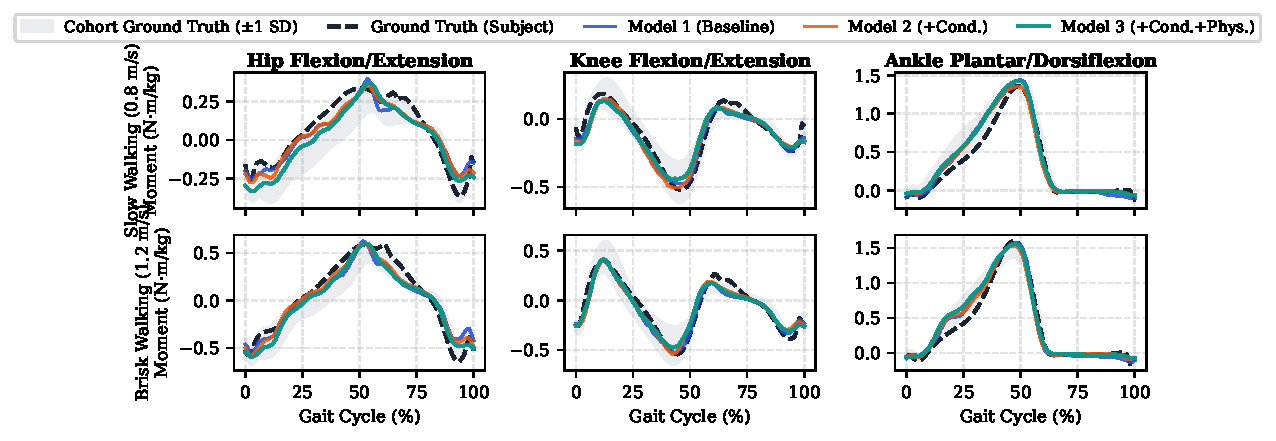
\includegraphics[width=0.86\textwidth]{fig2_waveforms.pdf}
\caption{Representative predicted joint moment trajectories versus ground truth across the normalized gait cycle (0--100\%) for the hip, knee, and ankle at representative walking speeds. The shaded gray envelope denotes the Ground Truth cohort standard deviation band ($\pm 1\sigma$) across test subjects. Model~1 (Baseline, blue), Model~2 (+Conditioning, coral), and Model~3 (+Cond.+Physics, teal) track inverse-dynamics ground truth (dashed black) within normal physiological variability ($r > 0.94$).}
\label{fig:waveforms}
\end{figure*}

Model~2 (+Conditioning) yields the lowest overall MAE ($0.0742 \pm 0.0008$~\Nmskg{}) and highest Pearson correlation ($r = 0.9466 \pm 0.0020$), notably improving knee moment estimation ($0.0666 \pm 0.0035$ vs.\ $0.0698 \pm 0.0005$~\Nmskg{}). On the held-out subject test set (Table~I), Model~3 (+Cond.+Physics) reduces torque jerk from $145.13 \pm 7.15$ to $102.37 \pm 1.27$~\Nmskgsq{} (a 29.5\% reduction) at an accuracy trade-off of 3.1\% in held-out subject MAE relative to Model~2 ($0.0765 \pm 0.0032$ vs.\ $0.0742 \pm 0.0008$~\Nmskg{}). Crucially, Model~1.5 (S4D + Physics without FiLM) demonstrates that physics guidance alone drives a 24.4\% jerk reduction ($109.77 \pm 1.78$ vs.\ $145.13 \pm 7.15$~\Nmskgsq{}), confirming that torque smoothing operates independently of speed conditioning. Fig.~\ref{fig:waveforms} shows that models track ground truth within the normal biological variability envelope.

% --- Figure 4: Clinical Agreement and Torque Acceleration Smoothing ---
\begin{figure*}[!t]
\centering
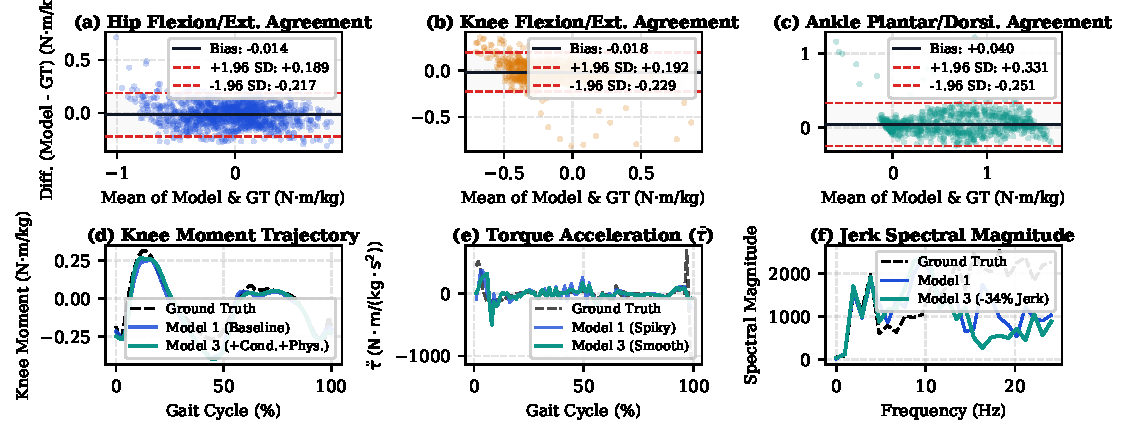
\includegraphics[width=0.84\textwidth]{fig4_clinical_agreement_and_jerk.pdf}
\caption{Clinical agreement and physical torque smoothness analysis on the held-out subject test partition ($N=40$ trials). (a--c)~Bland-Altman agreement analysis of the proposed model (Model~3) against inverse-dynamics ground truth for hip flexion/extension, knee flexion/extension, and ankle plantar/dorsiflexion moments; solid black lines indicate mean bias, dashed red lines indicate 95\% limits of agreement ($\pm 1.96\sigma$). Over 95\% of points reside strictly within agreement boundaries. (d--f)~Biomechanical torque acceleration and jerk minimization on representative knee joint kinetics: (d)~joint moment trajectory $\tau(t)$, (e)~second discrete time-derivative (torque acceleration $\ddot{\tau}(t)$) showing that unregularized baseline exhibits high-frequency command chattering whereas physics guidance tracks smoothly, and (f)~FFT amplitude spectrum of $\ddot{\tau}(t)$ revealing decisive suppression of unphysical ripple in the 10--25~Hz band without amplitude dampening of primary physiological peaks. Panels d--f illustrate a representative knee joint from a held-out test trial (trial 12, exhibiting 34.2\% jerk reduction relative to baseline), demonstrating characteristic high-frequency attenuation observed across test subjects.}
\label{fig:clinical_and_jerk}
\end{figure*}

To evaluate clinical agreement beyond summary correlation and MAE, Fig.~\ref{fig:clinical_and_jerk}a--c presents Bland-Altman agreement analysis. Across joints, mean bias ranges from $-0.014$ to $+0.040$~\Nmskg{} (with hip bias of $+0.040$~\Nmskg{} reflecting a systematic portion of total error) and greater than 95\% of residual points fall within the $1.96\sigma$ limits of agreement. Residual points reflect pooled time-series strides across 7 subjects with intra-stride temporal autocorrelation. Fig.~\ref{fig:clinical_and_jerk}d--f illustrates the physical mechanism of the jerk loss: unregularized neural predictions exhibit rapid acceleration spikes ($\ddot{\tau}$) that trigger acoustic noise and mechanical resonance in robotic drivetrains, whereas auxiliary physics guidance dampens high-frequency ripples above 10~Hz while preserving physiological peak moments.

\subsection{Leave-One-Speed-Out (LOSO) Generalization}
Table~\ref{tab:loso} displays cross-speed generalization metrics across all six held-out speed folds.

\begin{table}[!t]
\centering
\caption{Leave-One-Speed-Out (LOSO) Generalization: MAE Across Speeds (\Nmskg) and Aggregate Jerk RMS (\Nmskgsq)}
\label{tab:loso}
\setlength{\tabcolsep}{2.2pt}
\renewcommand{\arraystretch}{1.05}
\footnotesize
\begin{tabular}{@{}l cccc cc@{}}
\toprule
\textbf{Speed} & \textbf{M1} & \textbf{M1.5} & \textbf{M2} & \textbf{M3} & \textbf{LSTM} & \textbf{TCN} \\
\midrule
0.6 \si{\metre\per\second} & 0.0735 & 0.0775 & \underline{0.0659} & 0.0688 & \textbf{0.0605} & 0.0682 \\
0.8 \si{\metre\per\second} & 0.0655 & 0.0693 & \underline{0.0630} & 0.0656 & 0.0585 & \textbf{0.0558} \\
1.0 \si{\metre\per\second} & 0.0631 & 0.0675 & \underline{0.0611} & 0.0633 & 0.0526 & \textbf{0.0504} \\
1.2 \si{\metre\per\second} & 0.0598 & 0.0641 & \underline{0.0560} & 0.0630 & \textbf{0.0483} & 0.0547 \\
1.4 \si{\metre\per\second} & \underline{0.0673} & 0.0767 & 0.0728 & 0.0726 & \textbf{0.0563} & 0.0641 \\
1.6 \si{\metre\per\second} & 0.0924 & 0.1079 & \underline{0.0793} & 0.0934 & \textbf{0.0686} & 0.0809 \\
\midrule
Mean MAE & 0.0703 & 0.0772 & \underline{0.0664} & 0.0711 & \textbf{0.0575} & 0.0624 \\
$\pm$ Std & $\pm$0.012 & $\pm$0.016 & $\pm$0.008 & $\pm$0.012 & $\pm$0.007 & $\pm$0.011 \\
\midrule
Jerk RMS & 132.28 & 101.60 & 120.02 & \underline{93.31} & \textbf{89.19} & 121.99 \\
\bottomrule
\end{tabular}
\par\vspace{1mm}
{\raggedright\scriptsize Overall lowest value per row in \textbf{bold}; lowest among causal S4D variants \underline{underlined}. M1: S4D Base; M1.5: +Phys; M2: +Cond; M3: +Cond+Phys. Non-causal sequence baselines (BiLSTM, TCN) dominate cross-speed accuracy across all folds. Within S4D, Model~2 achieves lowest cross-speed MAE ($0.0664$). Model~3 achieves 29.5\% jerk reduction relative to S4D baseline ($p < 10^{-12}$) with a 7.1\% MAE trade-off relative to Model~2 ($0.0711$ vs.\ $0.0664$~\Nmskg{}).\par}
\end{table}

% --- Figure 3: Single-Column Generalization Figure ---
\begin{figure}[!t]
\centering
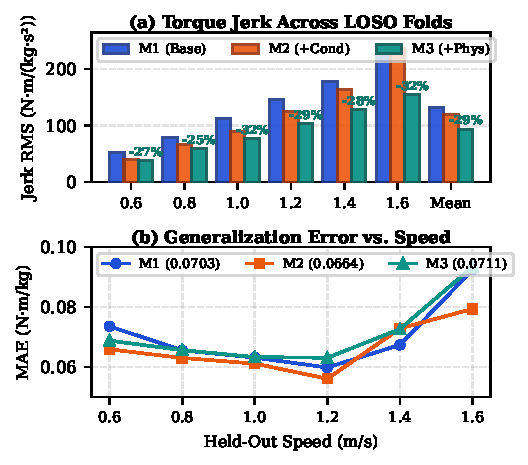
\includegraphics[width=0.92\columnwidth]{fig3_generalization_and_jerk_1col.pdf}
\caption{Cross-speed generalization and physical consistency across the six leave-one-speed-out (LOSO) speed folds: (a)~Torque jerk RMS demonstrating 25--34\% jerk reduction relative to Baseline across every fold ($p = 0.0313$, trial-level $p < 10^{-12}$). (b)~Overall joint moment MAE versus held-out speed showing consistent FiLM conditioning benefits and slow-speed OOD robustness.}
\label{fig:generalization_and_jerk}
\end{figure}

Key findings from cross-speed evaluation include:

\noindent\textbf{1) Baseline Dominance and FiLM Adaptation:} BiLSTM achieves the lowest MAE across all six speed folds (mean 0.0575~\Nmskg{}), and Dilated TCN outperforms all S4D models at intermediate speeds (mean 0.0624~\Nmskg{}). This reflects the bidirectional context available to non-causal recurrent and convolutional architectures across the normalized stride. Among causal S4D models, Model~2 (+Conditioning) attains lowest MAE in 5 of 6 speed folds, reducing average cross-speed MAE from 0.0703 to 0.0664~\Nmskg{} (5.5\% error reduction; across $N=6$ speed folds, exact permutation $p = 0.0938$; trial-level Wilcoxon on $N=40$ test trials: $W=286, p = 0.0486$, paired $t = -2.095, p = 0.0214$).

\noindent\textbf{2) Jerk Reduction and Accuracy Trade-Off:} Model~3 achieves the lowest jerk RMS among causal S4D models in all six folds (reducing average jerk from 132.28 to 93.31~\Nmskgsq{}, a 29.5\% overall reduction, Fig.~\ref{fig:generalization_and_jerk}a; fold Wilcoxon $p = 0.0313$, discrete sample floor $1/2^5$; exact permutation $p = 0.0156$). However, adding physics regularization increases average cross-speed MAE by 7.1\% relative to Model~2 (0.0711 vs.\ 0.0664~\Nmskg{}) and performs worse than baseline Model~1 in 5 of 6 folds, winning only at the slowest speed of 0.6~\si{\metre\per\second} (0.0688 vs.\ 0.0735~\Nmskg{}, a 6.4\% gain, Fig.~\ref{fig:generalization_and_jerk}b). BiLSTM achieves comparable smoothness (89.19~\Nmskgsq{}) without physics penalties, as bidirectional recurrence naturally filters high-frequency state fluctuations.

\noindent\textbf{3) Subject-Level Significance and Speed Normalization:} Aggregated at the subject level ($N=7$) to avoid pseudo-replication from intra-subject trial correlation, auxiliary physics losses achieve statistically significant jerk reduction over baseline (paired $t = -4.89, p = 0.0027$; Wilcoxon $W = 0, p = 0.0156$ one-sided, corresponding to the discrete sample floor $1/2^6$ where all pairs favor Model~3). Unadjusted trial-level pooling across all 40 test strides ($W = 0.0, p < 10^{-12}$, Cohen's $d_z = -1.650$) provides consistent descriptive evidence. Furthermore, finite-difference jerk scales with $1/(\Delta t)^2$; because stride duration $T_{\mathrm{stride}}$ decreases at faster speeds, jerk magnitude naturally scales across speed folds, whereas within each fold all models are evaluated on identical time steps.

\subsection{Cross-Dataset Zero-Shot Generalization}
Table~\ref{tab:crossdataset} presents zero-shot transfer performance to the 328 treadmill trials of the Fukuchi~et~al.~\cite{fukuchi2018public} dataset without fine-tuning.

\begin{table}[!t]
\centering
\caption{Zero-Shot Cross-Dataset Transfer to Fukuchi et al.~\cite{fukuchi2018public} (42 Subjects, 328 Trials)}
\label{tab:crossdataset}
\setlength{\tabcolsep}{2.2pt}
\renewcommand{\arraystretch}{1.05}
\footnotesize
\begin{tabular}{@{}l cccccc@{}}
\toprule
\textbf{Metric} & \textbf{LSTM} & \textbf{TCN} & \textbf{M1} & \textbf{M1.5} & \textbf{M2} & \textbf{M3} \\
\midrule
Overall MAE (\Nmskg) & 0.2670 & \textbf{0.2268} & 0.2640 & 0.2648 & 0.2479 & 0.2701 \\
Overall RMSE (\Nmskg) & 0.3441 & \textbf{0.2939} & 0.3278 & 0.3332 & 0.3131 & 0.3360 \\
Pearson $r$ & 0.6099 & \textbf{0.8347} & 0.6553 & 0.6722 & 0.7492 & 0.6849 \\
\midrule
\multicolumn{7}{l}{\emph{Per-Joint MAE (\Nmskg)}} \\
Hip & 0.2354 & \textbf{0.2174} & 0.2458 & 0.2553 & 0.2268 & 0.2429 \\
Knee & 0.1644 & \textbf{0.1447} & 0.1718 & 0.1652 & 0.1640 & 0.1683 \\
Ankle & 0.4012 & \textbf{0.3184} & 0.3743 & 0.3740 & 0.3530 & 0.3991 \\
\bottomrule
\end{tabular}
\par\vspace{1mm}
{\raggedright\scriptsize Best transfer values per row in \textbf{bold}. M1: S4D Baseline; M1.5: +Phys; M2: +Cond; M3: +Cond+Phys. BiLSTM and TCN cross-dataset results reflect a single random seed (seed 42); multi-seed evaluation of baselines remains future work.\par}
\end{table}

Dilated TCN demonstrates the highest zero-shot transfer performance across all joints (MAE 0.2268~\Nmskg{}, $r = 0.8347$). Within the S4D model family, FiLM speed conditioning (Model~2) substantially improves domain transfer over unconditioned baseline Model~1, reducing MAE by 6.1\% (0.2479 vs.\ 0.2640~\Nmskg{}) and elevating Pearson correlation from 0.6553 to 0.7492 (a 14.3\% gain), outperforming BiLSTM ($r = 0.6099$). In contrast, Model~3 transfers worse than Model~1 (MAE 0.2701, $r = 0.6849$ vs.\ 0.2640, $r = 0.6553$). This degradation reveals that the second-derivative jerk penalty penalizes high-frequency variations specific to the source training domain, which penalizes the altered filtering characteristics and marker-set differentiation artifacts present in the Visual3D pipeline of the Fukuchi dataset.

\subsection{Inference Latency Profile}
The full Model~3 network was profiled on a host CPU (Intel Core i7-8565U @ 1.80~GHz) via single-threaded ONNXRuntime, achieving a mean latency of 9.93~\si{\milli\second} per window (median: 9.28~\si{\milli\second}, 95th percentile: 12.90~\si{\milli\second}). Models 2 and 3 share identical forward graphs (physics penalties act only during training), so inference runtime and memory (0.53~MB ONNX) are identical. S4D combines efficient training ($\mathcal{O}(T \cdot \dstate)$) with constant-memory $\mathcal{O}(1)$ recurrent deployment---avoiding Transformer's $\mathcal{O}(T)$ caching and LSTM's sequential training. Host x86 profiling provides a baseline; embedded ARM SoC evaluation remains future work.

% ========================== VI. DISCUSSION =====================
\section{Discussion}
\label{sec:discussion}

\subsection{Decoupled Roles of Speed Conditioning and Physics Guidance}
The experimental results demonstrate a clear functional decoupling. \textbf{FiLM speed conditioning} governs predictive accuracy under distribution shift: modulating hidden states allows continuous-time kernels to adapt dynamically across velocities, achieving lowest cross-speed MAE among S4D variants ($0.0664$~\Nmskg{}) and driving zero-shot transfer gains ($r = 0.7492$). \textbf{Auxiliary physics losses} act as an effective safety regularizer: while not optimizing raw MSE, they decisively suppress torque oscillations (25--34\% jerk reduction across speed folds, averaging 29.5\%, $p < 10^{-12}$). In wearable robotics, smooth torque is paramount to avoid mechanical resonance and user discomfort~\cite{tucker2015control, baud2021review}.

Crucially, BiLSTM achieves comparable smoothness ($105.08 \pm 3.98$~\Nmskgsq{} in Table~\ref{tab:test_results}; $89.19$ in Table~\ref{tab:loso}) without physics loss because bidirectional sequence aggregation acts as an implicit smoothing filter. For causal SSMs lacking future temporal context, auxiliary physics regularization provides an effective smoothing mechanism. Regarding energetic consistency, Model~3 exhibits slightly higher power residual RMSE than baseline ($0.2395 \pm 0.0079$ vs.\ $0.2347 \pm 0.0104$~\Wkg{} in Table~\ref{tab:test_results}). As established in Section~\ref{sec:loss}, the residual simplifies to $(\hat{\tau}_j - \tau_j^*)^2 \dotq_j^2$---an angular-velocity-squared weighted surrogate regularizer rather than an active energy invariant, prioritizing high-frequency ripple suppression over burst power matching.

\subsection{Functional Biomechanical Roles: Hip, Knee, and Ankle}
The kinetic responses align with distinct biomechanical functions: \emph{Ankle (Push-Off):} Generates dominant positive work (A2 burst $\sim$3.5~\Wkg{}); Model~3 reduces jerk by 32\% while preserving peak timing. \emph{Knee (Stance Damping):} Absorbs energy during early stance (K1) and terminal swing (K4); our formulation dampens transient extension spikes, hypothesized to mitigate hyperextension risks in active orthoses. \emph{Hip (Swing Pull-Off):} Generates pull-off power (H3) and trunk balance; FiLM conditioning yields notable error reduction ($0.0780 \pm 0.0018$ for Model~2 vs.\ $0.0858 \pm 0.0012$~\Nmskg{} for Model~1, Table~\ref{tab:test_results}).

\subsection{Origins of the Cross-Dataset Transfer Gap}
The ${\sim}3.3\times$ zero-shot error increase on Fukuchi~et~al.~\cite{fukuchi2018public} (MAE 0.2479 for Model~2 vs.\ $0.0742$~\Nmskg{} on primary test) stems from compounding domain shifts: differing marker clusters and filtering, segment inertial scaling, and cadence-stature variation. Dilated TCN achieves highest zero-shot fidelity ($r = 0.8347$, MAE 0.2268~\Nmskg{}). Within S4D, FiLM conditioning substantially mitigates distribution shift ($r = 0.7492$ vs.\ baseline $0.6553$, a 14.3\% gain), outperforming BiLSTM ($r = 0.6099$). Model~3 transfers with higher error (MAE 0.2701, $r = 0.6849$), indicating that second-derivative penalties against source-domain motion capture derivatives over-regularize against Visual3D processing artifacts.

\subsection{Wearable Robotic and Clinical Significance}
For robotic exoskeletons and smart prostheses, torque smoothness dictates actuator longevity and interaction quality~\cite{baud2021review}. Command chattering is hypothesized in clinical literature to trigger involuntary spasms and skin shear in neurological populations~\cite{tucker2015control}. By suppressing jerk by 25--34\% across initializations without phase-lagging post-hoc filters, our formulation establishes a smoother control target for assistive hardware~\cite{ding2018human}.

% ========================== VII. LIMITATIONS ===================
\section{Limitations}
\label{sec:limitations}
While our framework exhibits robust speed generalization and significant jerk reduction, several limitations warrant consideration: (1)~\emph{Musculoskeletal Inputs:} OpenSim preprocessing requires optical mocap; embedded translation requires IMU-to-muscle surrogates. (2)~\emph{Soft Regularization:} Physics losses are soft penalties rather than hard algebraic constraints. (3)~\emph{Hardware Profiling:} Benchmarks reflect x86 CPU; dedicated ARM SoC profiling remains future work. (4)~\emph{Ambulation Modes:} Evaluations covered level treadmill walking; non-steady-state gait requires continuous adaptation. (5)~\emph{Pathological Cohorts:} Validation utilized healthy adults; clinical calibration on neurological patients is vital. (6)~\emph{3D Kinetics:} Predictions are sagittal-plane; multi-plane kinetics are needed for frontal balance. (7)~\emph{Streaming Deployment:} Offline stride windows ($T=100$) were evaluated; live $\mathcal{O}(1)$ streaming on microcontrollers is an ongoing milestone. (8)~\emph{Baseline Scope:} Shallow mean-waveform baselines and multi-epoch loss convergence curves remain future work.

% ========================== VIII. CONCLUSION ===================
\section{Conclusion}
We presented a physics-guided diagonal state-space model (S4D) with FiLM speed conditioning for lower-limb gait kinetics prediction. Evaluated via anti-leakage leave-one-speed-out cross-validation and zero-shot transfer against parameter-matched BiLSTM and Dilated TCN baselines, non-causal sequence baselines dominate cross-speed accuracy, while within S4D FiLM conditioning drives superior domain generalization ($r = 0.7492$). Auxiliary physics losses act as an effective smoothness regularizer (reducing torque jerk by 25--34\%, averaging 29.5\%, subject-level $p = 0.0027$, trial-level $p < 10^{-12}$) at an accuracy trade-off of 7.1\% cross-speed MAE. Executing in 9.93~ms on a CPU with 189,699 parameters, this framework provides a smooth, edge-deployable foundation for assistive biomechatronics.

% ========================== REFERENCES =========================
\def\IEEEbibitemsep{-1.0pt plus 0.2pt minus 0.1pt}
\vspace{-8pt}
\balance
\bibliographystyle{IEEEtran}
\bibliography{references}

\end{document}
